% Author: Philipp Moers <soziflip funny character gmail dot com>

\documentclass[12pt, oneside, a4paper, numbers=enddot, abstracton]{scrreprt}

\input{/home/flip/daten/latex/sfliptex05/sfliptex05.tex}

\begin{document}
\selectlanguage{english}

\begin{titlepage}
    \begin{center}
        \Large{Universität Tübingen}\\[1cm]
        \large{\scshape{SS 2014}}\\
        \large{\scshape{Torsten Grust, Alexander Ulrich}}\\[3cm]
        \Huge{\textbf{Functional Programming}}\\[6cm]
        \large{Notes from}\\[1cm]
        \large{Philipp Moers \\ <soziflip funnycharacter gmail dot com>}\\[3cm]
        \vfill
        \footnotesize{Last updated: \today, \currenttime}
    \end{center}
\end{titlepage}

\begin{abstract}
    This is just the product of me taking notes on the lecture. Nothing official. If you find mistakes or have got any questions, please feel free to contact me. Cheers!
\end{abstract}


\tableofcontents


\newpage

\vspace*{\fill}
»\textit{A programming language is a medium for expressing ideas (not to get a computer to perform operations) and only incidentally for machines to execute.}«\\
\begin{flushright}
    Harold Abelson and Gerald Jay Sussman
\end{flushright}
\vspace*{\fill}

\newpage


\section{Links}

Site: \url{http://db.inf.uni-tuebingen.de/teaching/FunctionalProgrammingSS2014.html}\\
Ilias: \url{http://goo.gl/rlqbkK}


\section{Literature}

\begin{itemize}
    \item Lipovača: \\ Learn You a Haskell for Great Good \\ No Starch Press 2011, \\ \url{http://learnyouahaskell.com}
    \item O'Sullivan, Steward, Goerzen: \\ Real World Haskell \\ O'Reilly 2010 \\ \url{http://book.realworldhaskell.org}
    \item Haskell 2010 Report, \\ \url{http://www.haskell.org/onlinereport/haskell2010}
\end{itemize}


% chapters:

%!TEX root = fp.tex

% Author: Philipp Moers <soziflip funny character gmail dot com>


\chapter{Introduction} % (fold)
\label{cha:introduction}

Computational model in Functional Programming: \textbf{reduction} (replace expression to values)

In Functional Programming, expressions are formed by applying functions to values.

\begin{enumerate}
    \item Functions as in math: $x = y \Rightarrow f(x) = f(y)$
    \item Functions are values (just like numbers, text \dots)
\end{enumerate}

\vspace{9pt}\begin{center}\begin{tabular}{|c|c|c|}\hline
\rowcolor{grau}                         & Functional                                & Imperative        \\\hline
                program construction    & function application and composition      & statement sequencing      \\\hline
                execution               & reduction (expression evaluation)         & state changes             \\\hline
                semantics               & lambda calculus                           & complex (denotational)    \\\hline
\end{tabular}\end{center}\vspace{9pt}

\newpage

\subsection*{Example}
$n \in \N, n \ge 2 $ is a prime number \textit{iff} the set of non-trivial factors is empty:\\
$$ n \text{ is prime} \Leftrightarrow \{\ m\ |\ m \in \{2,\dots, n-1\},\ n \mod m = 0 \} = \emptyset $$
\\
\codefile{haskell}{caption={isPrime.hs}, label=codefile:isPrime.hs}{../material/isPrime.hs}



% chapter introduction (end)


%!TEX root = fp.tex

% Author: Philipp Moers <soziflip funny character gmail dot com>

\chapter{Haskell Ramp-Up} % (fold)
\label{cha:haskell_ramp_up}

(Read $\equiv$ as ``denotes the same value as'')

\begin{itemize}
    \item Apply f to value e: \codeline{f e} (juxtaposition, ``apply'', binary operator \textvisiblespace, Haskell speak: infixL 10 \textvisiblespace)
    \item \textvisiblespace\ has max precedence (10): \codeline{f e$_1$ + e$_2$} $\equiv$ \codeline{(f e$_1$) + e$_2$}
    \item \textvisiblespace\ associates to the left: \codeline{g f e} $\equiv$ \codeline{(g f) e} \\ (\codeline{(g f)} is a function) \item Function composition: \begin{itemize}
        \item \codeline{( g . f ) e} $\equiv$ \codeline{g (f e)} \\ (. is something like mathematical $\circ$ ``after'')
        \item Alternative ``apply''-operator \codeline{\$} (lowest precedence, associates to the right, infixR $\emptyset\ \$$):\\
            \codeline{g \$ f \$ e} $\equiv$ \codeline{g \$ (f \$ e)} $\equiv$ \codeline{g (f e)}
        \item Prefix application of binary infix operator $\otimes$: \codeline{$(\otimes)$ e$_1$ e$_2$} $\equiv$ \codeline{e$_1$ $\otimes$ e$_2$} 
        \item Infix application of binary function f: \codeline{e$_1$ `f` e$_2$} $\equiv$ \codeline{f e$_1$ e$_2$}:
        \begin{itemize}
            \item \codeline{1 `elem` [1,2,3]}   ($1 \in \{1,2,3\}$)
            \item \codeline{n `mod` m}
            \item \dots
        \end{itemize}
        \item User defined operators, built from symbols \\ ! \# \$ \% \& * + / < = > ? \@ \textbackslash \string^ \textbar $\sim$:.
    \end{itemize}
\end{itemize} 


% chapter haskell_ramp_up (end)



%!TEX root = fp.tex

% Author: Philipp Moers <soziflip funny character gmail dot com>

\chapter{Values and Types} % (fold)
\label{cha:values_and_types}

Any Haskell expression e has a type t (\codeline{e :: t}) that is determined at compile time.
The \textbf{type assigmnent ::} is either given explicitly or inferred by the compiler.


\section{Base Types}

\vspace{9pt}\begin{center}\begin{tabular}{|c|c|c|}\hline
\rowcolor{grau}     Type            & Description                                   & values                                \\\hline
                    Int             & fixed-prec. integer                           & 0, 1, (-42)                           \\\hline
                    Integer         & arbitrary prec. integer                       & 10\textasciicircum 100                \\\hline
                    Float, Double   & single/double floating point (IEEE)           & 0.1, 1e02                             \\\hline
                    Char            & Unicode character                             & ``x'', ``\textbackslash t'', 
                                                                                        ``$\triangle$'', ``\textbackslash 8710''\\\hline
                    Bool            & Boolean                                       & True, False                           \\\hline
                    ()              & Unit                                          & ()                                    \\\hline
\end{tabular}\end{center}\vspace{9pt}


\section{Type Constructors}

\begin{itemize}
    \item Build new types from existing types
    \item Let a, b \dots denote arbitrary types (\textbf{type variables})
\end{itemize}

\vspace{9pt}\begin{center}\begin{tabular}{|c|c|c|}\hline
\rowcolor{grau}     Type            & Description                                   & values                        \\\hline
                    (a, b)          & pairs of values of type a, b                  & (1, True) :: (Int, Bool)      \\\hline
                    (a$_1$, a$_2$, \dots a$_n$) & n-tuples                          &                               \\\hline
                    [a]             & list of values of type a                      & [True, False] :: [Bool], []::[a]          \\\hline
                    Maybe a         & optional value of type a                      & \multirow{2}{3.7cm}{Just 42 :: Maybe Int 
                                                                                                         Nothing :: Maybe a}    \\
                                    &                                               &                               \\\hline
                    Either a b      & choice                                        & \multirow{2}{5cm}{Left ``x'' :: Either Char b
                                                                                                     Right pi :: Either a Double}   \\
                                    &                                               &                               \\\hline
                    IO a            & \multirow{2}{4.2cm}{I/O actions that 
                                                            return a value of type a}   & print 42 :: IO ()             \\
                                    &                                               &                               \\\hline
                    a ->\ b& functions from a to b                       & isLetter :: Char ->\ Bool      \\\hline
\end{tabular}\end{center}\vspace{9pt}


\section{Currying}

\begin{itemize}
  \item \textit{Recall}: \codeline{e$_1$ ++ e$_2$} $\equiv$ \codeline{(++) e$_1$ e$_2$}
  \item \codeline{(++) e$_1$ e$_2$} $\equiv$ \codeline{((++) e$_1$) e$_2$}
  \item Function application happens one argument at a time. \\ (\textbf{Currying}, Haskell B. Curry)
  \item Type of n-ary function is \\ a$_1$ -> a$_2$ -> \dots a$_n$ -> b
  \item Type fun -> associates to the right, read above type as \\ a$_1$ -> (a$_2$ -> (\dots ($a_n$ -> $b$)))
  \item Enables \textbf{Partial Application}
\end{itemize}


\section{Defining Values (and thus functions)}

\begin{itemize}
  \item \codeline{=} binds names to values. Names must not start with A-Z (Haskell style: camelCase)
  \item Define constant (0-ary function) c. Value of c is value of expression e. \\ \codeline{c = e}
  \item Define n-ary function f with arguments x$_i$. f may occur in e. \\ \codeline{f x$_1$ x$_2$ \dots x$_n$ = e}
  \item A Haskell program is a set of bindings.
  \item Good style: give type assigmnents for top-level (global) bindings: 
  \begin{codebox}[haskell]
f :: a@$_1$@ -> a@$_2$@ -> b
f x@$_1$@ x@$_2$@ = e
  \end{codebox}
\end{itemize}

\subsection{Guards}

Guards are conditional expressions (something like ``switch'' in Java).
They are a lot more readable and more powerful than \codeline{if \dots then \dots else \dots}.

Guards are introduced by \codeline{|}:
\begin{codebox}[haskell]
f x@$_1$@ x@$_2$@ @\dots@ x@$_n$@
  | q@$_1$@     = e@$_1$@
  | q@$_2$@     = e@$_2$@
  @\dots@
  | q@$_m$@     = e@$_m$@
[ | otherwise   = e@$_{m+1}$@ ]
\end{codebox}

Guards (q$_i$) are expressions of type Bool, evaluated top to bottom.

\codefile{haskell}{caption={factorial.hs}, label=factorial.hs}{../material/factorial.hs}



\subsection{Local Definitions}

\begin{enumerate}
  \item \textbf{Where bindings}: local definitions visible in the entire rhs of a definition.\\
  \begin{codebox}[haskell]
f@$_1$@ x@$_1$@ x@$_2$@ @\dots@ x@$_n$@ | q@$_1$@ = e@$_1$@
                    | q@$_2$@ = e@$_2$@ 
                    @\dots@
                    | q@$_m$@ = e@$_m$@ 
          where 
              g@$_1$@ = @\dots@
              g@$_2$@ = @\dots@
              @\dots@
              g@$_o$@
  \end{codebox}

  \codefile{haskell}{caption={power.hs}, label=power.hs}{../material/power.hs}

  \item \textbf{Let expressions}: local definitions visible inside one expression.\\
  \begin{codebox}[haskell]
let g@$_1$@ = @\dots@
    g@$_2$@ = @\dots@
    @\dots@
    g@$_o$@
in e
  \end{codebox}
\end{enumerate}


\subsection{Lists}

\begin{itemize}
  \item Recursive definitions:
  \begin{enumerate}
      \item \codeline{[]} is a list (nil), type [] :: [a]
      \item \codeline{x:xs} is a list, if x :: a, xs :: [a] \\ (x is head, xs is tail)
  \end{enumerate}
  \item Notation: \codeline{3:(2:(1:[]))} $\equiv$ \codeline{3:2:1:[]} $\equiv$ \codeline{[3,2,1]} $\equiv$ \codeline{3:[2,1]}
  \item Law: $\forall$ xs :: [a] :   \hspace{1cm} (xs $\neq$ []) \\
      \codeline{head xs : tail xs} == xs
\end{itemize}




\subsection{Pattern Matching}

\begin{itemize}
  \item \textit{The} idiomatic Haskell way to define a function by cases:
  \begin{codebox}[haskell]
f :: a@$_1$@ -> @\dots@ a@$_n$@ -> b
f p@$_11$@ @\dots@ p@$_1k$@ = e@$_1$@
f p@$_21$@ @\dots@ p@$_2k$@ = e@$_2$@
@\dots@
f p@$_n1$@ @\dots@ p@$_nk$@ = e@$_k$@
  \end{codebox}

\end{itemize}

\vspace{9pt}\begin{center}\begin{tabular}{|c|c|c|}\hline
\rowcolor{grau}   Pattern         & Matches If                & Bindings in e$_r$     \\\hline
                  constant c      & x$_i$ == c                  &                     \\\hline
                  variable v      & always                    & v $\equiv$ x$_i$      \\\hline
                  wildcard \_      & always                    &                       \\\hline
                  tuple (p$_1$, \dots p$_m$)  & components of x$_i$ match patterns p    & \\\hline
                  []              & x$_i$ == []                 &                     \\\hline
                  (p$_1$ : p$_2$)     & head x$_i$ matches p$_1$, tail x$_i$ matches p$_2$    & \\\hline
\end{tabular}\end{center}\vspace{9pt}


\codefile{haskell}{caption={tally.hs}, label=tally.hs}{../material/tally.hs}
\newpage
\codefile{haskell}{caption={take.hs}, label=take.hs}{../material/take.hs}
\codefile{haskell}{caption={mergesort.hs}, label=mergesort.hs}{../material/mergesort.hs}




\section{Algebraic Data Types}

(also known as \textbf{Sum-of-Product-Types})

\begin{itemize}
  \item \textit{Recall}: \codeline{[]} and \codeline{(:)} are the \textbf{values constructors} for \textbf{type constructor} [a]. 
  \item Can define entirely new type T and its constructors K$_i$:
        \begin{codebox}[haskell]
data T a@$_1$@ a@$_2$@ @\dots@ a@$_n$@ = K@$_1$@ b@$_{11}$@ @\dots@ b@$_{1_{n_1}}$@
                     K@$_2$@ b@$_{21}$@ @\dots@ b@$_{2_{n_2}}$@
                     @\dots@
                     K@$_r$@ b@$_{r1}$@ @\dots@ b@$_{r_{n_r}}$@
        \end{codebox}
        b$_{ij}$ types mentioning the type vars a$_1$ \dots a$_n$

  \item Defines type constructor T and r value constructors:\\
        \codeline{K$_i$ :: b$_{i_1}$ -> b$_{i_2}$ -> \dots b$_{in_i}$ -> T a$_1$ \dots a$_n$}
  \item Compare \codeline{[] :: [a]} and \codeline{(:) :: a -> [a] -> [a]}
  \item \textbf{Sum Type} (n=0, n$_i$ = 0) 
        \codefile{haskell}{caption={weekday.hs}, label=weekday.hs}{../material/weekday.hs}
  \item Add \codeline{deriving (c, c, \dots c)} to data declaration to define canonical operations: 
  \vspace{9pt}\begin{center}\begin{tabular}{|c|c|}\hline
  \rowcolor{grau} c       & operations                          \\\hline
                  Eq      & equality (==, /=)                   \\\hline
                  Show    & printing (show)                     \\\hline
                  Ord     & ordering (<, <=, max)               \\\hline
                  Enum    & enumeration                         \\\hline
                  Bounded & minBound, maxBound                  \\\hline
  \end{tabular}\end{center}\vspace{9pt}
  % \codefile{haskell}{caption={deriving.hs}, label=deriving.hs}{../material/deriving.hs}
  \item \textbf{Product Types} (r=1)
  \codefile{haskell}{caption={sequence.hs}, label=sequence.hs}{../material/sequence.hs}
  \item \textbf{Sum-of-Product-Types}\\
    \codeline{data Maybe a = Just a | Nothing}\\
    \codeline{data Either a b = Left a | Right b}\\
    \codeline{data List a = Nil | Cons a (List a)}
    \codefile{haskell}{caption={cons.hs}, label=cons.hs}{../material/cons.hs}
    \textit{Anschauung zu liftList:}
    % List a  - fromList ->   [a]
    % | g                     ^ 
    % v                       | g''
    % List b  - toList  ->    [b]
    \begin{center} 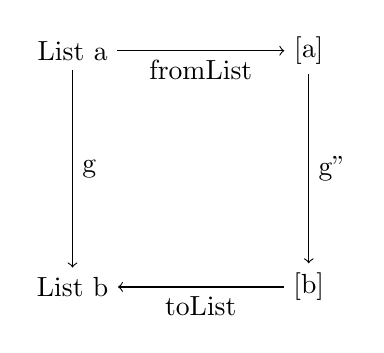
\begin{tikzpicture}[node distance = 3cm]
      \node                     (lista) {List a};
      \node [below of = lista]   (listb) {List b};
      \node [right of = lista]   (la) {[a]};
      \node [right of = listb]   (lb) {[b]};
      \path[->] (lista) edge[right] node[below] {fromList} (la)
                (lb) edge[right] node[below] {toList} (listb)
                (lista) edge[below] node[right] {g} (listb)
                (la) edge[below] node[right] {g''} (lb)
      ;
    \end{tikzpicture} \end{center}

  \codefile{haskell}{caption={eval-compile-run.hs}, label=eval-compile-run.hs}{../material/eval-compile-run.hs}
  \item \textit{Erläuterung zur Super-simple stack machine}:\\
    \begin{itemize}
      \item ``push'' pushes a new element to the stack
      \item ``DoAdd'' substitutes the first two elements of the stack with their sum
    \end{itemize}

        
\end{itemize}





% chapter values_and_types (end)






%!TEX root = fp.tex

% Author: Philipp Moers <soziflip funny character gmail dot com>

\chapter{Type Classes} % (fold)
\label{cha:type_classes}

A \textbf{type class} C defines a family of type signatures („methods“) which all \textbf{instances} of C must implement.

\begin{codebox}[haskell]
class C a where
    f@$_1$@ :: t@$_1$@
    @\dots@
    f@$_n$@ :: t@$_n$@
\end{codebox}
The \codeline{t$_i$} \underline{must} mention a.\\
For any \codeline{f$_i$} the class may provide default implementations. \\
We have \codeline{f$_i$ :: C a => t$_i$} \\ (read „if a is instance C then f$_i$ has type t$_i$“).\\
\codeline{C a} is called \textbf{class constraint}.

\textit{Example}:

\begin{codebox}[haskell]
class Eq a where
    (==) :: a -> a -> Bool
    (/=) :: a -> a -> Bool
    x == y = not (x /= y)
    x /= y = not (x == y)
\end{codebox}
(These are default implementations. To redefine one of them is sufficient.)

\codefile{haskell}{caption={type-classes.hs}, label=type-classes.hs}{../material/type-classes.hs}


\section{Class Inheritance}

\begin{itemize}
    \item Defining \codeline{class (c$_1$ a, c$_2$ a, \dots) => C a where \dots} makes type class C a subclass of the C$_i$.\\
    \item \codeline{C a => t} implies \codeline{C$_1$ a, C$_2$ a \dots}.
\end{itemize}

\vspace{9pt}
% \includegraphics[scale=1.0]{type-class-inheritance.png}
\textcolor{myorange}{[Here is an image missing]}
\vspace{9pt}


\section{Class Instances}

If type t implements the methods of class C, t becomes an \textbf{instance of} C:
\begin{codebox}[haskell]
instance C t where
    f@$_1$@ = <def of f@$_1$@>
    @\dots@
    f@$_n$@ = <def of f@$_n$@>
\end{codebox}
(All defs of f$_i$ may be provided, minimal complete definition \underline{must} be provided.)
Class constraint C t is satisfied from now on.

\textit{Example}:

\begin{codebox}[haskell]
instance Eq Bool where
    x == y = x && y || (not x && not y)
\end{codebox}

An instance definition for type constructor t may formulate class constraints for its argument types a, b, \dots:\\
\codeline{instance (C$_1$ a, C$_2$ a, \dots) => C t where}


\codefile{haskell}{caption={rock-paper-scissor-inst.hs}, label=rock-paper-scissor-inst.hs}{../material/rock-paper-scissor-inst.hs}


\subsection{Deriving Class Instances}

Automatically make user-defined data types (\codeline{data \dots}) instances of classes C$_i$ $\in$ \{ Eq, Ord, Enum, Bounded, Show, Read \}:

\begin{codebox}[haskell]
data T a@$_1$@ a@$_1$@ @\dots@ a@$_n$@ = @\dots@
                   | @\dots@
    deriving (C@$_1$@, C@$_2$@, @\dots@)
\end{codebox}

\codefile{haskell}{caption={rock-paper-scissor-inst-deriving.hs}, label=rock-paper-scissor-inst-deriving.hs}{../material/rock-paper-scissor-inst-deriving.hs}




% chapter type_classes (end)


%!TEX root = fp.tex

% Author: Philipp Moers <soziflip funny character gmail dot com>


\chapter{Domain-Specific Languages} % (fold)
\label{cha:domain_specific_languages}
a.k.a. \textbf{DSLs}

\begin{itemize}
    \item ``small'''' languages designed to easily and directly express the concepts/idioms of a specific domain. \underline{Not} turing-complete in general.
    \item Examples:
        \vspace{9pt}\begin{center}\begin{tabular}{|c|c|}\hline
        \rowcolor{grau} Domain          & DSLs                                  \\\hline
                        OS automation   & shell scripts, OSX Automater          \\\hline
                        Typesetting     & \LaTeX                                \\\hline
                        Queries         & SQL                                   \\\hline
                        Game Scripting  & Unreal Script, Lua                    \\\hline
                        Parsing         & Yacc, Bison, ANTLR                    \\\hline
        \end{tabular}\end{center}\vspace{9pt}
    \item Functional Languages make good hosts for \textbf{embedded DSLs}:
        \begin{itemize}
            \item algebraic datatypes (e.g. to model ASTs)
            \item higher-order functions (abstractionn, control constructs)
            \item lightweight syntax (layout / whitespace, non-alphabetic ids)
        \end{itemize}
\end{itemize}


\newpage

\textit{Example}: An embedded DSL for integer sets:
\begin{codebox}[haskell]
type IntegerSet = 
    -- constructors:
    empty :: IntegerSet
    insert :: Integer -> IntegerSet -> IntegerSet
    delete :: Integer -> IntegerSet -> IntegerSet
    -- observer:
    member :: Integer -> IntegerSet -> Bool

member 3 (insert 1 (delete 3 (insert 2 (insert 3 empty))))
    @$\equiv$@ False
\end{codebox}

\vspace{2cm}

\textbf{(1)}
DSL as library of functions, implementation details exposed. 

\vspace{9pt}
% TODO encode unicode chars!!!
% \codefile{haskell}{caption={library-exposed.hs}, label=library-exposed.hs}{../material/library-exposed.hs}
\textcolor{myorange}{[Here is library-exposed.hs missing!]}
\vspace{9pt}



\section{Modules}

\begin{itemize}
    \item Group of related definitions (values, types) in a single file \\ (named ``M.hs'' / ``M.lhs''):
    \begin{codebox}[haskell]
module M where
    type Predicate a = a -> Bool
    id :: a -> a
    id x = x
    \end{codebox}
    \item Hierarchy: module A.B.C.M in file A/B/C/M.hs
    \item Access definitions in other module M:
    \begin{codebox}[haskell]
import M
    \end{codebox}

    \newpage
    \item Explicit export lists hide all other definitions:
    \begin{codebox}[haskell]
module M (id) where
    ...
    -- type Predicate a not exported
    \end{codebox}
    \item \textbf{Abstract data types}:\\
    export algebraic data types, but \underline{not} its constructors:
        \begin{codebox}[haskell]
module M (Rose, leaf) where
    data Rose a = Node a [Rose a]
    leaf :: a -> Rose a [Rose a]
    leaf x = Node x []
        \end{codebox}
    \begin{itemize}
        \item Export constructors:
        \begin{codebox}[haskell]
module M (Rose(Node), leaf) where
    @\dots@
-- or export all constructors:
module M (Rose(..), leaf) where
        \end{codebox}
        \item Instance definitions (including deriving) are exported with their type.
    \end{itemize}
    \item Qualified imports to partition name space:
    \begin{codebox}[haskell]
import qualified M
    ...
    -- use M.foobar syntax
    t :: M.Rose Char
    t = M.leaf 'x'
    \end{codebox}
    \item Partially import module:
    \begin{codebox}[haskell]
-- only import nub and reverse
import Data.List (nub, reverse)

-- import whole module but without otherwise
import Prelude hiding (otherwise)
otherwise :: Bool
otherwise = False -- harhar
    \end{codebox}
    \item Pass imported modules to importer of own module:
    \begin{codebox}[haskell]
module M (..., module Data.List, ...) where
    import Data.List (nub)
    \end{codebox}
    \begin{codebox}[haskell]
import qualified M
    M.nub
    \end{codebox}
\end{itemize}

% \codefile{haskell}{caption={SetLanguage.hs}, label=SetLanguage.hs}{../material/SetLanguage.hs}
% \codefile{haskell}{caption={SetLanguageShallow.hs}, label=SetLanguageShallow.hs}{../material/SetLanguageShallow.hs}
\codefile{haskell}{caption={SetLanguageShallowCard.hs}, label=SetLanguageShallowCard.hs}{../material/SetLanguageShallowCard.hs}
\codefile{haskell}{caption={set-language-shallow.hs}, label=set-language-shallow.hs}{../material/set-language-shallow.hs}


\vspace{2cm}

\textbf{(2)}
DSL as library of functions, abstract data type (module).
\begin{itemize}
    \item \textbf{Shallow DSL embedding}:\\
    Semantics of DSL operations directly expressed in terms of host language value (e.g. list or characteristic function)
    \begin{itemize}
        \item constructors (empty, insert, delete) perform the work, harder to add
        \item observers (member) trivial
    \end{itemize}
    \item \textbf{Deep DSL embedding}:\\
    DSL operations build an abstract syntax tree (AST) that represents applications and arguments
    \begin{itemize}
        \item constructors merely build the AST, very easy to add
        \item observers interpret (traverse) the AST and perform the work
    \end{itemize}
    % \codefile{haskell}{caption={SetLanguageDeep.hs}, label=SetLanguageDeep.hs}{../material/SetLanguageDeep.hs}
    \codefile{haskell}{caption={SetLanguageDeepCard.hs}, label=SetLanguageDeepCard.hs}{../material/SetLanguageDeepCard.hs}
    \codefile{haskell}{caption={set-language-deep.hs}, label=set-language-deep.hs}{../material/set-language-deep.hs}

\end{itemize}

\newpage 

\codefile{haskell}{caption={ExprDeepNum.hs}, label={ExprDeepNum.hs}}{../material/ExprDeepNum.hs}
\codefile{haskell}{caption={expr-deep-num.hs}, label={expr-deep-num.hs}}{../material/expr-deep-num.hs}

% \codefile{haskell}{caption={expr-language.hs}, label={expr-language.hs}}{../material/expr-language.hs}


% \codefile{haskell}{caption={ExprDeep.hs}, label={ExprDeep.hs}}{../material/ExprDeep.hs}
% \codefile{haskell}{caption={ExprDeepGADTUntyped.hs}, label={ExprDeepGADTUntyped.hs}}{../material/ExprDeepGADTUntyped.hs}



\section{Generalized Algebraic Data Types (GADTs)}

\textit{Idea}: 
\begin{itemize}
    \item Encode the type of a DSL expression (here: Integer or Bool) in its \textbf{Haskell representation type}.
    \item Use Haskell's type checker to ensure at compile time that only well-typed DSL expressions are built.
\end{itemize}

\textit{Language extensions:}\\
\codeline{\{-\# LANGUAGE GADTs \#-\}}
\begin{itemize}
    \item Define new parameterized type T, its constructors k$_i$ and their type signatures:
    \begin{codebox}[haskell]
data T a@$_1$@ a@$_2$@ @\dots@ a@$_n$@ where
    k@$_1$@ :: b@$_{11}$@ -> @\dots@ -> b@$_1n_1$@ -> T t@$_{11}$@ t@$_{1n}$@
    @\dots@
    k@$_r$@ :: b@$_{r1}$@ -> @\dots@ -> b@$_rn_r$@ -> T t@$_{r1}$@ t@$_{rn}$@
    \end{codebox}
\end{itemize}

\codefile{haskell}{caption={ExprDeepGADTTyped.hs}, label={ExprDeepGADTTyped.hs}}{../material/ExprDeepGADTTyped.hs_ASCII}
\codefile{haskell}{caption={expr-language-typed.hs}, label={expr-language-typed.hs}}{../material/expr-language-typed.hs}

% \codefile{haskell}{caption={ExprShallow.hs}, label={ExprShallow.hs}}{../material/ExprShallow.hs}
% \codefile{haskell}{caption={expr-language-shallow.hs}, label={expr-language-shallow.hs}}{../material/expr-language-shallow.hs}
\codefile{haskell}{caption={ExprShallowPrint.hs}, label={ExprShallowPrint.hs}}{../material/ExprShallowPrint.hs}
\codefile{haskell}{caption={expr-language-shallow-print.hs}, label={expr-language-shallow-print.hs}}{../material/expr-language-shallow-print.hs}



\section{Shallow embedding of a String Matching DSL}

\begin{itemize}
    \item \textbf{Pattern}:
    \begin{enumerate}
        \item Given a String, a pattern returns the list of matches. Match failure? Returns the empty list.
        \item A match consists of a value (e.g. the matched characters, tokens, parse trees) and the residual String left to match.
    \end{enumerate}
    Thus: \codeline{type Pattern a = String -> [(a, String)]}
\end{itemize}

\subsection{DSL design}
\vspace{9pt}\begin{center}\begin{tabular}{|c|c|c|}\hline
\rowcolor{grau} Pattern                 &               & DSL function     \\\hline
                match lit. char         & "x"           & \codeline{lit :: Char -> Pattern Char}    \\\hline
                match empty string      & $\epsilon$    & \codeline{empty :: a -> Pattern a}        \\\hline
                fail always             & $\emptyset$   & \codeline{fail :: Pattern a}              \\\hline
                alternative             & |             & \parbox[t]{9cm}{\codeline{alt :: Pattern a ->} \\ \codeline{Pattern a -> Pattern a}}  \\\hline
                sequence                & .             & \parbox[t]{9cm}{\codeline{seq :: (a -> b -> c) ->} \\ \codeline{Pattern a -> Pattern b -> Pattern c}} \\\hline
                repitition              & *             & \codeline{rep :: Pattern a -> Pattern [a]} \\\hline
\end{tabular}\end{center}\vspace{9pt}

% \codefile{haskell}{caption={PatternMatch.hs}, label={PatternMatch.hs}}{./PatternMatch.hs}
% \codefile{haskell}{caption={pattern-match.hs}, label={pattern-match.hs}}{./pattern-match.hs}
\codefile{haskell}{caption={PatternMatching.hs}, label={PatternMatching.hs}}{../material/PatternMatching.hs}
\codefile{haskell}{caption={simple-patterns.hs}, label={simple-patterns.hs}}{../material/simple-patterns.hs}

\codefile{haskell}{caption={pattern-matching.hs}, label={pattern-matching.hs}}{../material/pattern-matching.hs}












% chapter domain_specific_languages (end)


% \input{chapter06-}


\end{document}
